\documentclass{article}
\usepackage{amsmath} % For mathematical formatting
\usepackage{tikz}    % For drawing diagrams
\usetikzlibrary{matrix, positioning} % For matrix nodes and positioning

\begin{document}

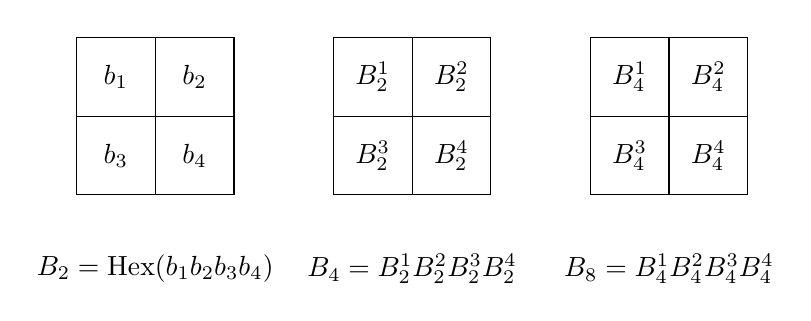
\begin{tikzpicture}[node distance=1cm]
    % Define styles for the grids
    \tikzset{
        mygrid/.style={
            matrix of math nodes,
            nodes={draw, minimum size=1cm, anchor=center},
            column sep=-\pgflinewidth,
            row sep=-\pgflinewidth
        }
    }

    % First section: 2x2 grid of bits
    \matrix (bits) [mygrid] {
        |(b1)| b_1 & |(b2)| b_2 \\
        |(b3)| b_3 & |(b4)| b_4 \\
    };
    \node[below=0.5cm of bits] {$B_2 = \text{Hex}(b_1 b_2 b_3 b_4)$};

    % Second section: 2x2 grid of B_2 blocks
    \matrix (blocks2) [mygrid, right=of bits] {
        |(B21)| B_2^1 & |(B22)| B_2^2 \\
        |(B23)| B_2^3 & |(B24)| B_2^4 \\
    };
    \node[below=0.5cm of blocks2] {$B_4 = B_2^1 B_2^2 B_2^3 B_2^4$};

    % Third section: 2x2 grid of B_4 blocks
    \matrix (blocks4) [mygrid, right=of blocks2] {
        |(B41)| B_4^1 & |(B42)| B_4^2 \\
        |(B43)| B_4^3 & |(B44)| B_4^4 \\
    };
    \node[below=0.5cm of blocks4] {$B_8 = B_4^1 B_4^2 B_4^3 B_4^4$};
\end{tikzpicture}

\end{document}